\chapter{Deep Multi-task Models for Histopathology}
\label{chapter:InvestigatedApproach}

We identified two different types of MT approaches in the field of Histopathology when it comes to the types of combined learning procedures. The more common one comes in the form of a MT network which learns through two or more supervised objectives. In the other class of approaches a supervised task is taught simultaneously with a self-supervised or even unsupervised one. The former is described in \textbf{Section \ref{hsmm}}, while \textbf{Section \ref{ssshmm}} present the latter class of intelligent algorithms.

\section{Fully Supervised
Multitask Models}
\label{hsmm}

We classify approaches which combine multiple supervised tasks based on nature of the combined objectives. Most MT networks perform two or more classification in the same time. These type of approaches will be presented in \textbf{Subsection \ref{classification_mt}}. In \textbf{Subsection \ref{classification_reg_mt}} we present a technique which combines a classification objective with a regression problem. We continue by describing intelligent techniques which perform multiple segmentation's simultaneously or a segmentation accompanied by another Image-to-Image inference in \textbf{Subsection \ref{segmentatiopn_mt}}. The last subsection from this section, \textbf{Subsection \ref{class_recog_mt}} analysis methods which fuse classification and segmentation. We decide to also include classification-detection hybrids in this part, as both segmentation and detection act as a localization and recognition tool.

\section{Multi-task Classification Models}
\label{classification_mt}
A pioneering work from the field  was introduced in \cite{bayramoglu2016deep}, where histological breast cancer images are classified as benign or malignant. This early MT approach, is also taught to predict the magnification factor. The resulting parallel architecture performs similarly to its single class equivalent showcasing that even early MT approaches allowed for the combination of multiple tasks without loss in performance. 

As deep learning matured, the performance of Multi-task models continued to improve. Early approaches including the previous one evolved from simple binary-classification between benign and malignant tissue to fine-grained multi-class classification of the cancer cells as is the case with the intelligent algorithm proposed in \cite{li2020multi}. Furthermore, their proposed parallel MT network also predicts the severity of breast cancer through the other classification head which classifies the tissue's grade in one of three classes. For the first objective, this method was able to achieve state-of-the-art results reaching a test accuracy of around 93.43\%.

One limitation in the Digital Pathology space when compared with other areas in which AI showed impressive results is the lack of large, medical datasets which would allow \textbf{Transfer Learning (TL)}. Pre-training on ImageNet \cite{deng2009imagenet} allows networks to learn many valuable features for many other classification problems. The sheer size of it also made the dataset the choice even in the medical field, although it contains no medical image. In order to fill this gap in medical Computer-Vision, the authors of \cite{mormont2020multi} propose a Multi-task approach able to aggregate the information from almost 90,000 images from 22 datasets. A common encoder is connected to 22 task-specific fully-connected layers, each tasked with classifying images from one of the datasets resulting in another parallel MT architecture. The learning objective is to reduce the mean loss obtained by averaging all the individual task-specific loss functions. A scheme of the model can be observed in \textbf{Figure \ref{mt_pretaining}}. The authors experimented with two established network backbones: ResNet50 \cite{he2016deep} and DenseNet121 \cite{huang2017densely}. Between the two, the first one performs better and improves the results when compared to ImageNet pre-training in almost all scenarios. The most significant increase is achieved in bone marrow classification exceeding the pre-existing pre-training method by around 6\%.

\begin{figure}[htb]
    \centering
	\centerline{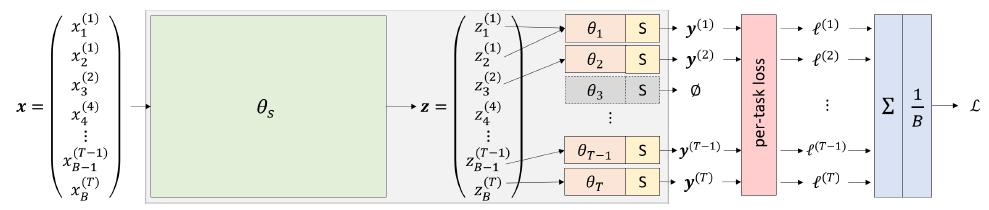
\includegraphics[scale=0.85]{figures/mt_pretraining.png}}
	\caption{The proposed MT arhitecture for pre-training on 22 datasets. Image from \cite{mormont2020multi}}
	\label{mt_pretaining}
\end{figure}

Recently, researchers employed multi-modal data in tandem with multi-task architecture in order to further develop the performance of existing approaches. One such approach was introduced in \cite{fan2022framework}. In this case, the multi-modality comes from the use of multi-parametric MRI images, a specific type of MRI which yields multiple types of medical data which better reflects the patient's state. The proposed network receives two inputs: the dynamic contrast-enhanced magnetic resonance images \textbf{(DCE-MRI)} and T2-weighted images \textbf{(T2WI}. Each has the benefit of better evidentiating complementary morphological characteristics of the human body. Starting from the ImageNet weights through the process of transfer learning, this multi-task network based of the VGG16 \cite{simonyan2014very} architecture learns to classify three cancer descriptors for breast cancer diagnosis: Luminal A, the histological grande and the Ki-67 expression. An illustration of the framework proposed in \cite{fan2022framework} is showcased in \textbf{Figure \ref{multimodal_multitask}}.

\begin{figure}[htb]
    \centering
	\centerline{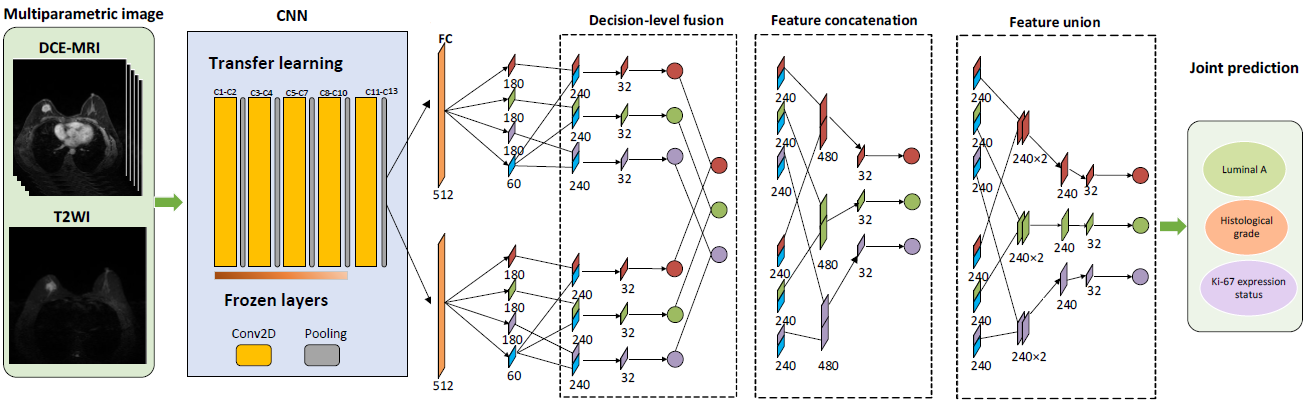
\includegraphics[scale=0.65]{figures/multimodal_multitask.png}}
	\caption{Multi-modal multi-task architecture for Luminal A, Histological Grade and Ki-67 expression status classification. Image adapted from from \cite{fan2022framework}}
	\label{multimodal_multitask}
\end{figure}

\section{Multi-task Model for Classification and Regression}
\label{classification_reg_mt}
Recently, researchers employed multi-modal data in tandem with Multi-task architecture in order to further develop the performance of existing approaches. One such approach was introduced in \cite{tan2022multi}. The proposed parallel Multi-task network receives two inputs: region of interests \textbf{(ROIs)} crops from a whole slide image \textbf{(WSI)} and mRNA expression data. The model dubbed, Multi-task
correlation learning \textbf{(MultiCoFusion)}, performs a classification task, in the form of cancer grade prediction in brain tissue and a regression task. The latter requires the network to predict the patient's survival risk. Unlike the previously described methods, MultiCoFusion does not have a single encoder. The multi-modality is processed through two different networks: ResNet152 for the histological images and a \textbf{Sparse Graph Neural Network (SGNN)} \cite{tan2021hierarchical} for the mRNA data. The extracted features are fused and passed to a Multi-task module which extract the most relevant features. Lastly one prediction heads is added for each task. Another unique aspect of this approach is the use of alternate learning instead of joint training, meaning that the network is updated based on only one objective for each batch. In this case, the determining objective is alternated after every batch.  An illustration of the proposed framework is showcased in \textbf{Figure \ref{multimodal_multitask2}}. MultiCoFusion is able to exceed all previous approaches, establishing itself as the state-of-the-art approach in both tasks.

\begin{figure}[htb]
    \centering
	\centerline{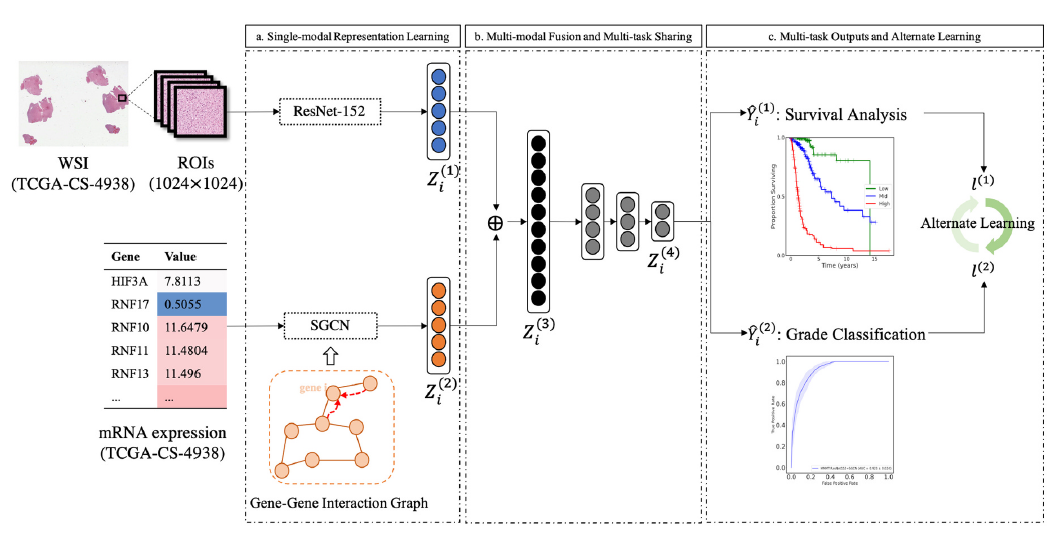
\includegraphics[scale=0.8]{figures/multimodal_multitask2.png}}
	\caption{MultiCoFusion architecture from \cite{tan2022multi}}
	\label{multimodal_multitask2}
\end{figure}

\section{Multi-task Segmentation Models}
\label{segmentatiopn_mt}

Another series of approaches combine two or more segmentation tasks in their MTL pipeline. Approaches \cite{wang2021bend} and \cite{rezazadeh2023multi} reformulate a single segmentation problem into a multi-objective one. The former approaches nuclei instance segmentation, while the latter tackles gland instance segmentation. In both problems, the entity instances overlap making a fine segmentation difficult resulting in a lower than desired performance. 

In both frameworks the instance segmentation is transformed in three segmentation objectives. Besides the original segmentation task, the researchers add adjacent objective which facilitate the separation of overlapping instances. In \cite{wang2021bend}, a nuclei distance map and the overlapping segmentation are performed in order to guide the main task. In \cite{rezazadeh2023multi}, the second segmentation head performs contour segmentation, while the third is tasked with overlapped gland segmentation, in a similar manner with the previous approach. 

The approach from \cite{wang2021bend}, named Bend-Net has an U-Net \cite{ronneberger2015u} structure with three decoders and gets its name from the novel proposed bending loss function. This objective is also proposed to deal with wrongly segmented overlapped nuclei. This is achieved by finding convex and concave points and the retrieved structures. Concave points are drastically penalized as they suggest the wrong merge of two independent entities. An example of how bending loss is computed can be observed in the following figure, \textbf{Figure \ref{bendingloss}}.

\begin{figure}[htb]
    \centering
	\centerline{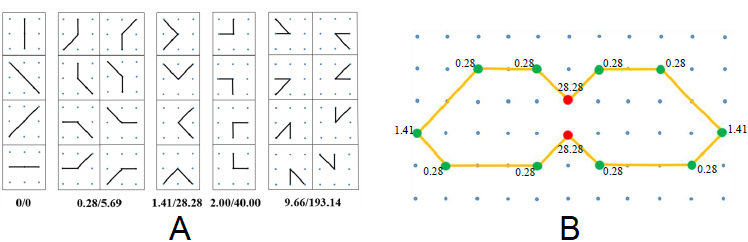
\includegraphics[scale=1]{figures/bend_loss.png}}
	\caption{(A) Examples of bending losses for different "curves". The same curve has a different score depending on wheter or not is seen as concave or convex. The values are presented as "convex score / concave score". (B) Example of bending loss computation for a given shape. \textcolor{forestgreen}{Green} indicates a convex point, whereas \textcolor{red}{red} indicates a concave point. Images from \cite{wang2021bend}. }
	\label{bendingloss}
\end{figure}

The Multi-task architecture combined with the bending loss outperforms numerous established networks in this task. Some results can be observed in \textbf{Figure \ref{bend_results}}

\begin{figure}[htb]
    \centering
	\centerline{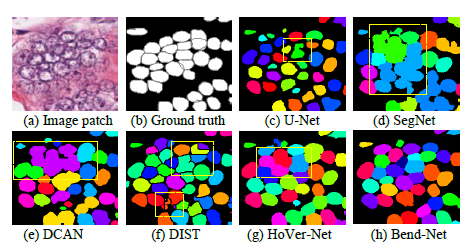
\includegraphics[scale=1]{figures/bend_results.png}}
	\caption{Inference example of nuclei instance segmentation for multiple neural networks. Image from \cite{wang2021bend}}
	\label{bend_results}
\end{figure}

In \cite{rezazadeh2023multi}, the authors demonstrate the effective of their proposed MT approach over the original starting point networks (DeepLabV3+ \cite{chen2018encoder} and U-Net). Through classic computer vision approach, starting from the instance segmentation ground-truth, they are able to obtain the contours segmentation map and the overlapping map, which in turn will be used as ground-truth in the MT pipeline. 

\begin{figure}[htb]
    \centering
	\centerline{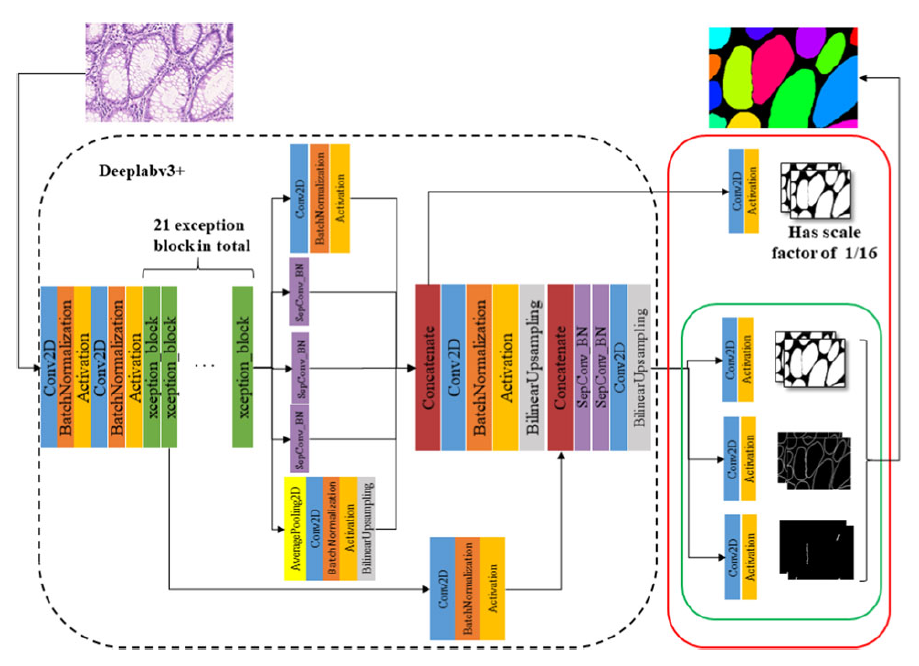
\includegraphics[scale=0.9]{figures/mt_deeplab.png}}
	\caption{Scheme of MT-DeepLab and MT-DeepLab-2 architectures from \cite{rezazadeh2023multi}. The black rounded rectangular encapsulated the DeepLabV3 network. The \textcolor{forestgreen}{green} area contains the MT-DeepLab components, while the \textcolor{red}{red} one also encapsulated the deeply-supervised MT-DeepLab-2 objective.}
	\label{mt_deeplab}
\end{figure}

The resulting network which performs the three segmentation tasks is simply named MT-DeepLab. As a way to continue the improvement of this model in the second version of the architecture, MT-DeepLab-2, a forth segmentation task is added. The model is encouraged to learn the segmentation map as soon as possible through the addition of this forth objectives which computes the instance segmentation loss at the start of the decoding path. Because the feature map has not yet gone through upsampling, this computation is done at a scale factor of 1/16. This type of learning is called Deep Supervision \cite{lee2015deeply}. Depending on the chosen metric either the first of the second MT-DeepLab outperform all other networks which were considered for the task of gland segmentation.

\section{Multi-task Models for Joint Classification and Recognition}
\label{class_recog_mt}

In \cite{yu2021large} a dataset for gastric cancer screening and localization is introduced. Furthermore, a MT network based on Deep Layer Aggregation is proposed \cite{yu2018deep}. Deformable convolutions \cite{dai2017deformable} are added to the model as many areas from WSIs contains little to no information, while other are densely packed with dense information. The method jointly learns to perform screening, a binary-classification problem in which tissue is classified as either normal or cancerous and semantic segmentation. The second task has the purpose of identifying the suspect areas in order to provide a justification for the diagnostic which could be verified by a doctor thus all cancerous cells have to be identified. 

\begin{figure}[htb]
    \centering
	\centerline{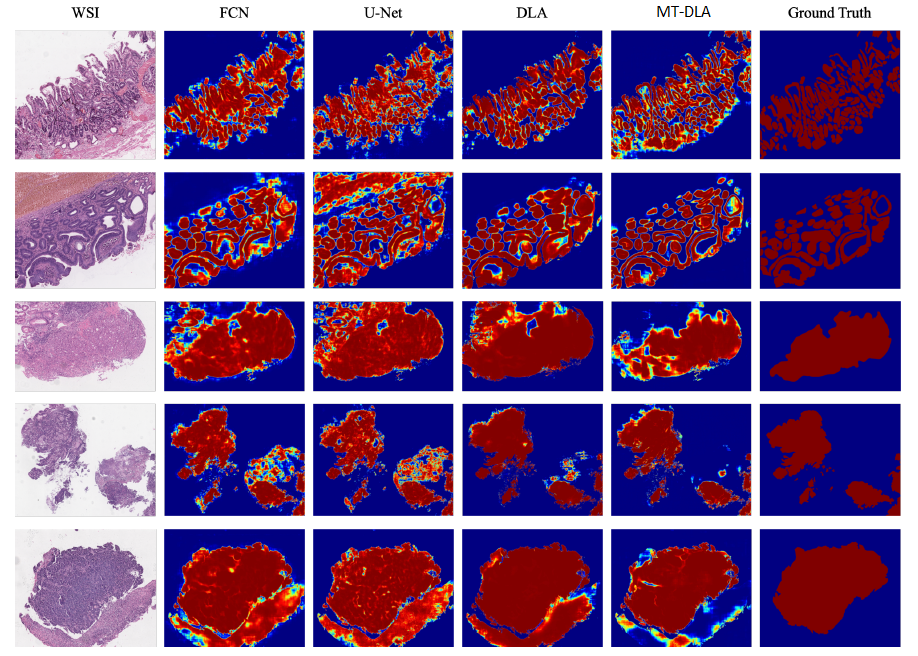
\includegraphics[scale=0.8]{figures/mtdla_results.png}}
	\caption{Predictions obtained by various networks for gastric cancer segmentation. Image from \cite{yu2021large}.}
	\label{mtdla_results}
\end{figure}

The proposed network, to which we will refer to as \textbf{Multi-Task Deep Layer Aggregation (MT-DLA)} achieves state-of-the-art results when compared with existing segmentation networks outperforming all candidates when it comes to both the segmentation and screening objective. The only metric in which the model is outperformed is specificity, which is not as relevant when it comes to identifying a dangerous disease in patients. Some results for the segmentation task can be seen in \textbf{Figure \ref{mtdla_results}}.

Paper \cite{dabass2022mtu} includes another Multi-task model which combines classification and segmentation, but unlike the previous approach it is applied for colon cancer. As many other networks which perform classification in a MTL environment in the field of Histopathology, the proposed network \textbf{Multi-Task U-Net (MTU)} classifies the tumour into either benign or malignant. Similar to the previous method, the segmentation is used to localize dangerous areas from the tissue. The design of this network is illustrated in \textbf{Figure \ref{mtu}}.

\begin{figure}[htb]
    \centering
	\centerline{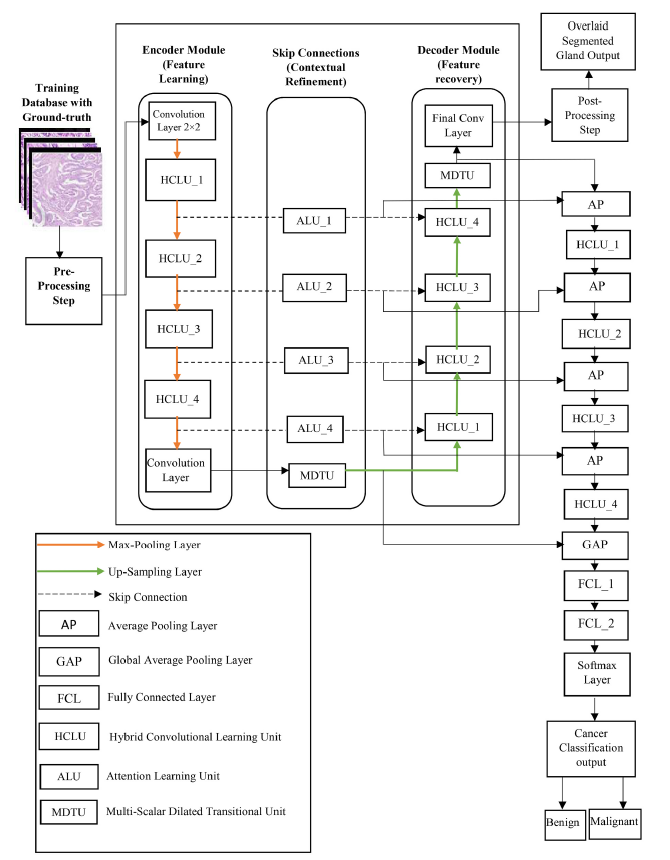
\includegraphics[scale=0.8]{figures/mtu.png}}
	\caption{MTU arhitecture diagram. Image from \cite{dabass2022mtu}}
	\label{mtu}
\end{figure}


Besides the addition of these additional objective, MTU also employs attention modules \cite{vaswani2017attention}. Another defining characteristic of the proposed approach is a novel block of layers design especially for WSIs, dubbed \textbf{Hybrid Convolutional Learning Unit (HCLU)}. The illustration of HCLU is showcased in \textbf{Figure \ref{hclu}}. This series of operations is a fusion between a Multi-Scalar Atrous Convolution, a Multi-Level Convolution and a Residual Block. The \textbf{Multi-Scalar Dilated Transitional Unit (MDTU)} is another newly introduced block which combines the results of four Atrous Convolutions with different dilation rates (1, 4, 8, 12). The features are aggregated through a \textbf{Global Average Pooling (GAP)} module. MTU was tested on two datasets, outperforming all its competitor.

\begin{figure}[htb]
    \centering
	\centerline{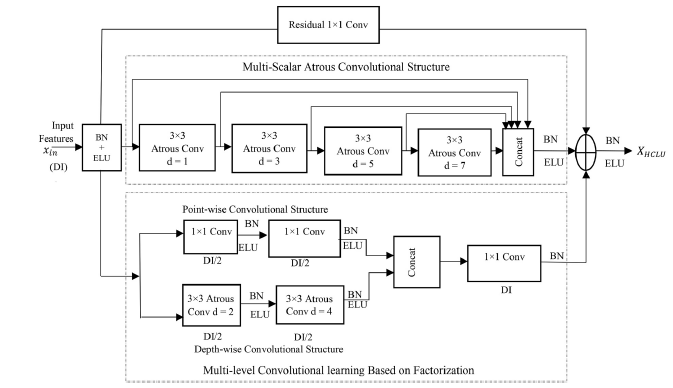
\includegraphics[scale=1]{figures/hclu.png}}
	\caption{HCLU block design. Image from \cite{dabass2022mtu}}
	\label{hclu}
\end{figure}

Similar to the work conducted in \cite{crawshaw2020multi}, paper \cite{graham2023one} introduces a MT network for processing different types of entities: nuclei, glands, tissue and lumen. The proposed model, named Cerberus. employs a common encoder which feeds data to three parallel decoders tasked with segmentation (nuclei, glands, lumen) and a module forth parallel module for tissue type classification. This allows the encoder, built following the structure of ResNet34, to learn rich features from multiple heterogeneous datasets, addressing data scarcity. U-Net like decoders are constructed for the segmentation tasks. The model achieves state-of-the-art-results exceeding the accuracy of other models in gland segmentation by almost 8\% and in lumen segmentation by around 10\%. An overview of the proposed framework is displayed in \textbf{Figure \ref{cerberus}}.

To further demonstrate the effectiveness of the encoder and their Multi-task learning strategy, the backbone is also used in two other transfer learning experiments. First of all, the pre-trained Cerberus encoder is used for the classification of nuclei. Next, the backbone is also employed in a detection task. Through the addition of object detection specific blocks which follow the RetinaNet \cite{lin2017focal} architecture, the model is able to learn to detect Signet ring cells. In nuclear classification, the pre-trained backbones yield a 4.6\% improvement on the test dataset when compared to previous approaches. It must be noted that in this experiments the pre-trained backbone is fully frozen.

Lastly, the authors tackle the of object subtyping. In this task, the segmented cell is further classified into four finer labels. As in the previous experiment the rest of the network is frozen, while the newly introduced decoder is taught to perform the multi-class segmentation. In all the experiments, Cerberus is shown to be a powerful network due to its encoder's ability to extract general, high-quality features.

\begin{figure}[htb]
    \centering
	\centerline{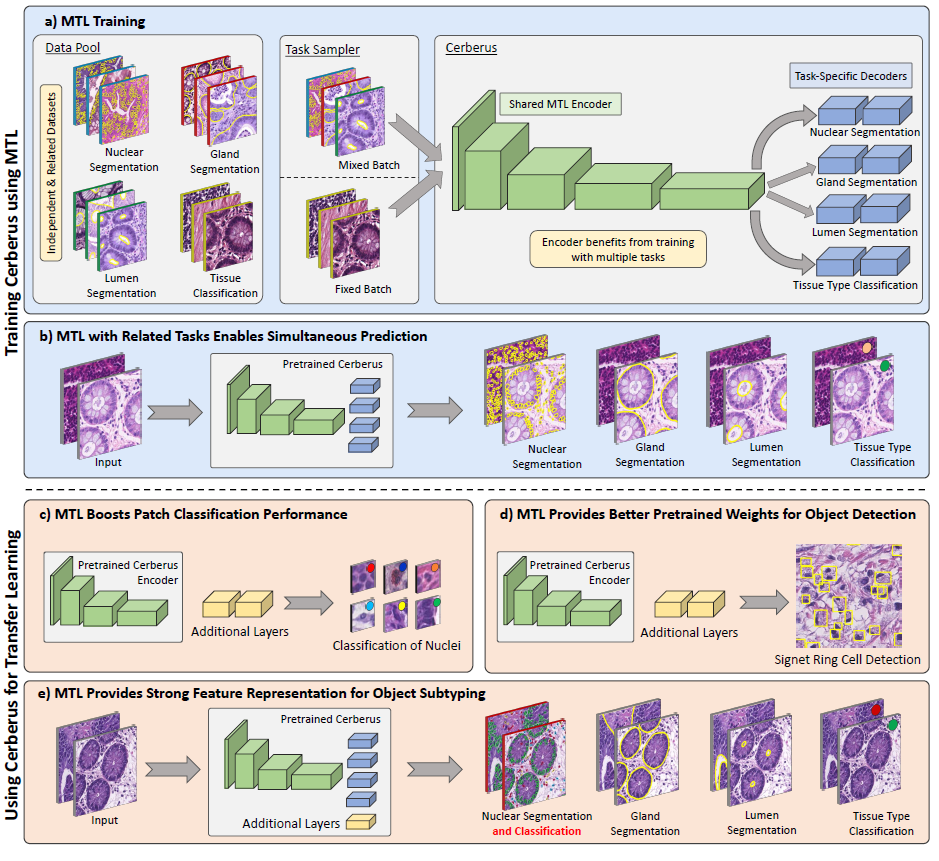
\includegraphics[scale=0.9]{figures/12.png}}
	\caption{Cerberus framework overview. Image from \cite{dabass2022mtu}}
	\label{cerberus}
\end{figure}

section{Supervised-Self-Supervised Hybrid Multitask Models}
label{ssshmm}

Reconstruction + Classification
cite{tellez2020extending}

Similarity + Image Reconstruction
cite{marik2022supervision}




